\section{Computational experiments}\label{sec:exp}
\subsection{Test cases and experimental settings}\label{sec:cases}
We evaluate the approach on three cases of different scales (\cref{tab:cases}). The small-scale case is a generated line with 5 stations and 30 trains of two types. The medium- and large-scale cases contain 12 stations with 60 trains and 29 stations with 101 trains, respectively, on lines of 172.1 and 1320~km. The cases differ not only in size but also in the density of their constraints: the medium-scale case has 75 station service frequency rules and 1855 route headway records, and the large-scale case has 2929 train operations with 1449 optional stops and 8047 route headway records.

\begin{table}[tb]
\centering\small
\caption{Characteristics of the test cases (computed from the input data).}\label{tab:cases}
\setlength{\tabcolsep}{4pt}
\begin{tabular}{@{}>{\raggedright\arraybackslash}p{78mm}rrr@{}}\toprule
 & Small & Medium & Large\\\midrule
Stations / sections & 5 / 4 & 12 / 11 & 29 / 28\\
Line length (km) & 66.0 & 172.1 & 1320.0\\
Trains / train types & 30 / 2 & 60 / 1 & 101 / 1\\
Train operations at stations & 150 & 685 & 2929\\
\quad mandatory stops / optional / mandatory passes & 62/88/0 & 120/445/120 & 288/1449/1192\\
Station tracks / receiving and departure routes & 16 / 24 & 63 / 173 & 195 / 493\\
Route headway records & 144 & 1855 & 8047\\
Station service frequency rules / train stop-count rules & 6 / 30 & 75 / 60 & 21 / 101\\
Maintenance window records / maximum travel time rules & 8 / 30 & 22 / 1 & 56 / 32\\
Time limit (h) & 1 & 6 & 6\\\bottomrule
\end{tabular}
\end{table}

The CD-ALNS is compared with two benchmarks. \emph{Direct MILP} solves the full MILP \eqref{eq:model} with the window classification \eqref{eq:freqlin} by Gurobi, minimizing $S$, $P$, and $R$ in sequence. \emph{LBBD} adapts the decomposition of \citet{Leutwiler2022} to the operating rules and data considered here: a macroscopic master problem determines times and stops, and station subproblems check platforming and return logical feasibility cuts. Its results therefore describe this adaptation rather than the original implementation. LBBD terminates at its first jointly feasible timetable, whereas CD-ALNS continues to improve the timetable. All solutions are checked against the same original constraints, including the exact service counting \eqref{eq:freq}. \Cref{tab:size} reports the sizes of the full MILP solved by Direct MILP, taken from the solver logs; they illustrate why the full model becomes impractical as the number of operations per station grows.

\begin{table}[tb]
\centering\small
\caption{Size of the full MILP (Gurobi log of Direct MILP, before presolve).}\label{tab:size}
\begin{tabular}{@{}lrrrr@{}}\toprule
Case & Constraints & Variables & Binary variables & Nonzeros\\\midrule
Small-scale & 74\,497 & 11\,009 & 4\,445 & 327\,305\\
Medium-scale & 990\,153 & 159\,979 & 111\,621 & 4\,504\,111\\
Large-scale & 13\,996\,162 & 1\,071\,296 & 701\,533 & 67\,266\,880\\\bottomrule
\end{tabular}
\end{table}

The algorithms are implemented in C\# on .NET 8 and use Gurobi 10.0.1 for all MILP and LP models. All experiments, including the benchmarks and the ablation, were performed on the same hardware with Intel Xeon E7-4850 v4 processors, using four threads. The time limit is one hour for the small-scale case and six hours for the other cases, and every run in this section uses one random seed. The parameters of the CD-ALNS are listed in \cref{tab:params}.

\subsection{Comparison of solution methods}\label{sec:compare}
We compare solution quality using the timetable makespan $S$, the preferred-window deviation penalty $P$, and the total running time supplement $R$ (\cref{tab:results}). Computation times record the first joint feasibility $t_{\mathrm{feas}}$, the first attainment of the best timetable makespan $t_{\mathrm{best}}$, and the total runtime $t_{\mathrm{run}}$. A dash and the status ``No joint solution'' indicate that no jointly feasible timetable was found before termination; this does not prove infeasibility.

\begin{table}[tb]
\centering\small
\caption{Computational results ($S$, $R$, and times in seconds; $P$ in weighted seconds).}\label{tab:results}
\footnotesize\setlength{\tabcolsep}{3.2pt}
\begin{tabular}{@{}llrrrrrrl@{}}\toprule
Case & Method & $S$ & $P$ & $R$ & $t_{\mathrm{feas}}$ & $t_{\mathrm{best}}$ & $t_{\mathrm{run}}$ & Status\\\midrule
Small-scale & CD-ALNS & 11\,385 & 0 & 0 & 10.41 & 76.64 & 3425.94 & Feasible\\
 & Direct MILP & 11\,385 & 0 & 0 & 35.67 & 35.67 & 56.08 & Makespan optimal\\
 & LBBD & 11\,385 & 0 & 0 & 1227.68 & 1227.68 & 1227.68 & Feasible\\\midrule
Medium-scale & CD-ALNS & 54\,525 & 272\,686 & 1926 & 428.89 & 4823.61 & 21\,026.71 & Feasible\\
 & Direct MILP & -- & -- & -- & -- & -- & 21\,007.85 & No joint solution\\
 & LBBD & -- & -- & -- & -- & -- & 21\,014.79 & No joint solution\\\midrule
Large-scale & CD-ALNS & 65\,849 & 3\,910\,668 & 4946 & 5199.39 & 15\,305.02 & 21\,121.28 & Feasible\\
 & Direct MILP & -- & -- & -- & -- & -- & 21\,092.48 & No joint solution\\
 & LBBD & -- & -- & -- & -- & -- & 21\,148.95 & No joint solution\\\bottomrule
\end{tabular}
\end{table}

In the small-scale case, all three methods attain the timetable makespan of 11\,385~s, which Direct MILP proves to be optimal. CD-ALNS finds joint feasibility first; Direct MILP attains the optimum earlier and has the shortest total runtime. For the medium-scale case, CD-ALNS finds joint feasibility at 428.89~s and reduces the timetable makespan from 59\,970 to 54\,525~s (9.08\%). Neither benchmark finds joint feasibility under the six-hour budget: Direct MILP finds no incumbent, and LBBD remains at its first master problem. For the large-scale case, CD-ALNS attains macroscopic and joint feasibility at 2467.08 and 5199.39~s, respectively, and reduces the timetable makespan from 68\,975 to 65\,849~s (4.53\%). Neither benchmark finds a jointly feasible timetable; LBBD completes one master iteration without an incumbent. These outcomes reflect the difficulty of obtaining a feasible master or full-model solution rather than the quality of the Benders cuts. Without valid lower bounds for the medium- and large-scale cases, the CD-ALNS optimality gaps remain unknown.

\subsection{Convergence analysis}\label{sec:convergence}
To examine feasibility restoration, we follow the medium-scale run in \cref{fig:restoration}. Initially, 84 macroscopic diagnostic conditions are violated (78 headway, four section-order, and two overtaking-cap conditions), with 20 long dwells without overtaking counted separately. Round 1 produces no candidate; round 2 reduces the counts to 23 and 4, and round 3 removes both. The macroscopically feasible timetable still contains nine conflicting station-operation pairs with a 2515~s aggregate separation deficit, although all section headways, which are lower bounds on the route headways, are satisfied. Joint repair removes both in nine rounds.

\begin{figure}[tb]
\centering
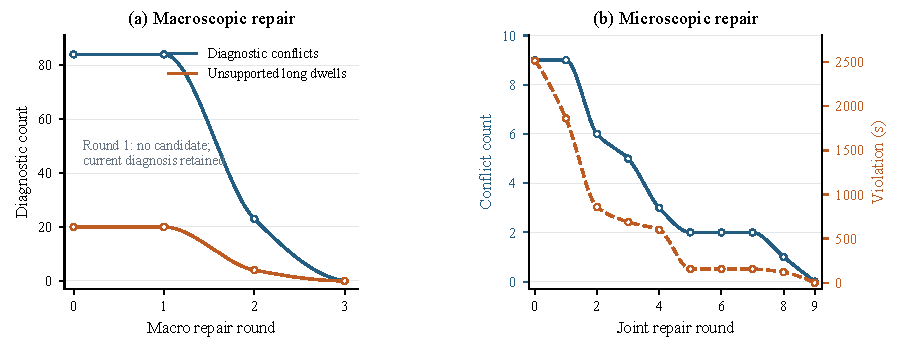
\includegraphics[width=0.86\textwidth]{figures/fig4_restoration.pdf}
\caption{Feasibility restoration in the medium-scale case: (a) violated macroscopic diagnostic conditions and long dwells without overtaking; (b) conflicting station-operation pairs and their aggregate temporal violation score. Round 0 gives the initial diagnosis.}\label{fig:restoration}
\end{figure}

After joint feasibility is reached, the timetable makespan is reduced further (\cref{fig:makespan}). In the small-scale case, the CD-ALNS reaches the optimal timetable makespan after two reductions. In the medium-scale case, the makespan decreases through eight improvements, seven of which occur within the first hour; in the large-scale case it decreases through four improvements. In the large-scale case, the first fixed-structure timetable re-optimization reduces the makespan from 68\,975 to 66\,929~s, i.e., by about two thirds of the total reduction, which illustrates the value of moving all event times of a structure together (\cref{prop:longest}).

\begin{figure}[tb]
\centering
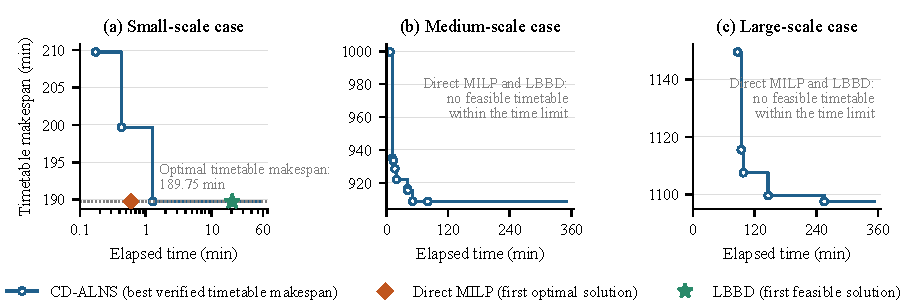
\includegraphics[width=\textwidth]{figures/fig5_makespan.pdf}
\caption{Best verified timetable makespan during optimization. The small-scale case uses a logarithmic time axis; each curve ends at the termination of its run.}\label{fig:makespan}
\end{figure}

\subsection{Analysis of the obtained timetables}\label{sec:solution}
\Cref{fig:solution} shows the best timetable of the medium-scale case and the track occupation at its busiest intermediate station. The 60 trains are accommodated between 06:33 and 21:41:45, i.e., within the makespan of 908.75~min, and overtaking takes place at several intermediate stations, visible as longer horizontal segments of the overtaken trains. Station S3 serves 25 intermediate stops on three tracks; in the period shown in \cref{fig:solution}(b), the stops are spread over two arrival--departure tracks, while passing trains use the main track. The time--distance diagram of the large-scale case is given in \cref{app:large}.

\begin{figure}[tb]
\centering
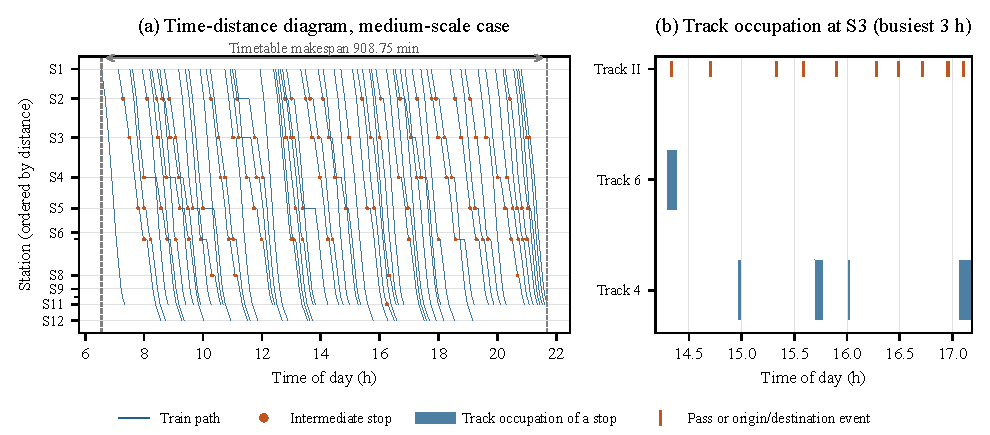
\includegraphics[width=\textwidth]{figures/fig_solution_medium.pdf}
\caption{Best jointly feasible timetable of the medium-scale case: (a) time--distance diagram, with stops marked; (b) track occupation at station S3 in its busiest three-hour period. Stations are numbered along the line.}\label{fig:solution}
\end{figure}

\Cref{tab:solution} summarizes the stopping and resource use of the best timetables, recounted from the saved solutions under the exact rule \eqref{eq:freq}. All service frequency requirements are satisfied, and many of them are binding: in the medium-scale case, 44 of the 75 station rules are exactly at their lower bound, and the average count exceeds the lower bound by only 0.59 stops. Binding service requirements are the situation in which a stop cannot be removed to resolve a conflict without compensation elsewhere, which is what the joint neighborhoods of \cref{sec:joint} provide.

\begin{table}[tb]
\centering\small
\caption{Stopping and station resource use of the best timetables.}\label{tab:solution}
\begin{tabular}{@{}lrrr@{}}\toprule
 & Small & Medium & Large\\\midrule
Intermediate operations / intermediate stops & 90 / 50 & 565 / 113 & 2727 / 707\\
Optional stops: available / used & 88 / 48 & 445 / 113 & 1449 / 621\\
Station service frequency rules & 6 & 75 & 21\\
\quad at lower bound / at upper bound / violated & 6 / 6 / 0 & 44 / 0 / 0 & 5 / 5 / 0\\
\quad average count above lower bound & 0.00 & 0.59 & 20.57\\
Station tracks used / available & 14 / 16 & 31 / 63 & 112 / 195\\\bottomrule
\end{tabular}
\end{table}

\subsection{Effect of the macroscopic ALNS phase}\label{sec:ablation}
To examine the role of the macroscopic ALNS, the ablation replaces it with the rule-based bounded repair of the initialization procedure, retaining the joint ALNS and identical data, objectives, time limit, joint settings, seed, solver, and hardware. In this paired medium-scale run (\cref{fig:ablation}), the full configuration reaches macroscopic and joint feasibility at 128.37 and 428.89~s, versus 2709.69 and 3159.98~s. It also reaches the shared final timetable makespan of 54\,525~s earlier (4823.61 versus 6039.26~s). The ablated configuration has lower final secondary objectives ($P=233\,464$, $R=933$~s, versus 272\,686 and 1926~s); the full configuration therefore does not improve every objective. Its macroscopic phase ends after three rounds, before the first weight update, so this observed improvement precedes adaptive weight learning and stems from the conflict-driven macroscopic operators.

\begin{figure}[tb]
\centering
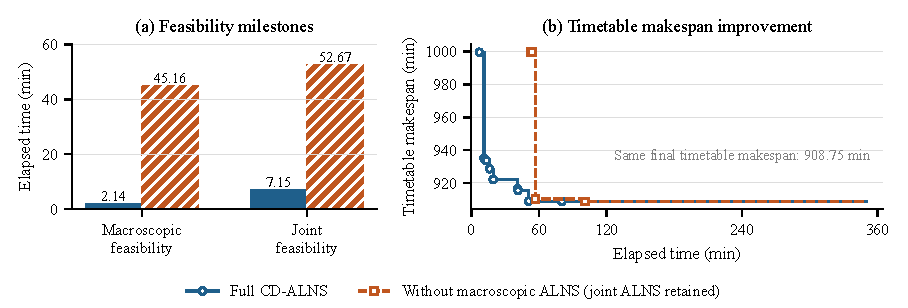
\includegraphics[width=\textwidth]{figures/fig6_ablation.pdf}
\caption{Effect of the macroscopic ALNS phase in the medium-scale case: (a) times to macroscopic and joint feasibility; (b) timetable makespan improvement. Both configurations attain the same timetable makespan of 908.75 min.}\label{fig:ablation}
\end{figure}

\subsection{Robustness over random seeds}\label{sec:seeds}
\begin{pending}[: E1, repeated runs]
Run CD-ALNS with 10 random seeds on each case (same time limits, hardware, and Gurobi version) and report, for $S$, $t_{\mathrm{feas}}$, and $t_{\mathrm{best}}$, the best, mean, worst, and standard deviation, and the number of runs that reach joint feasibility. Fill \cref{tab:seeds} and add box plots of $S$ and $t_{\mathrm{feas}}$.
\end{pending}
\begin{table}[htbp]
\centering\small
\caption{Results of CD-ALNS over 10 random seeds (to be completed).}\label{tab:seeds}
\begin{tabular}{@{}lccccccc@{}}\toprule
Case & Feasible runs & $S$ best & $S$ mean & $S$ worst & $S$ std. & $t_{\mathrm{feas}}$ mean & $t_{\mathrm{best}}$ mean\\\midrule
Small-scale & \tbd & \tbd & \tbd & \tbd & \tbd & \tbd & \tbd\\
Medium-scale & \tbd & \tbd & \tbd & \tbd & \tbd & \tbd & \tbd\\
Large-scale & \tbd & \tbd & \tbd & \tbd & \tbd & \tbd & \tbd\\\bottomrule
\end{tabular}
\end{table}

\subsection{Contribution of the algorithmic components}\label{sec:components}
\begin{pending}[: E2, component ablations and operator statistics]
On the medium- and large-scale cases (several seeds each), compare the full CD-ALNS with: (i) without J3 service frequency compensation; (ii) without J4 boundary extension; (iii) without J5 tight temporal links; (iv) uniform random operator selection instead of adaptive weights; (v) without fixed-structure re-optimization; (vi) a standard LNS with random destroy of trains and the same MILP repair. Report $S$, $t_{\mathrm{feas}}$, and $t_{\mathrm{best}}$ in \cref{tab:components}. In addition, report the selection frequency, success rate, and average time of each operator and scale per phase (from the iteration logs), e.g., as a heat map.
\end{pending}
\begin{table}[htbp]
\centering\small
\caption{Component ablations (to be completed; mean over seeds).}\label{tab:components}
\footnotesize\setlength{\tabcolsep}{4pt}
\begin{tabular}{@{}lcccccc@{}}\toprule
 & \multicolumn{3}{c}{Medium-scale} & \multicolumn{3}{c}{Large-scale}\\\cmidrule(lr){2-4}\cmidrule(l){5-7}
Configuration & $S$ & $t_{\mathrm{feas}}$ & $t_{\mathrm{best}}$ & $S$ & $t_{\mathrm{feas}}$ & $t_{\mathrm{best}}$\\\midrule
Full CD-ALNS & \tbd & \tbd & \tbd & \tbd & \tbd & \tbd\\
Without J3 (frequency compensation) & \tbd & \tbd & \tbd & \tbd & \tbd & \tbd\\
Without J4 (boundary) & \tbd & \tbd & \tbd & \tbd & \tbd & \tbd\\
Without J5 (tight temporal links) & \tbd & \tbd & \tbd & \tbd & \tbd & \tbd\\
Uniform operator selection & \tbd & \tbd & \tbd & \tbd & \tbd & \tbd\\
Without fixed-structure re-optimization & \tbd & \tbd & \tbd & \tbd & \tbd & \tbd\\
Standard LNS (random destroy, MILP repair) & \tbd & \tbd & \tbd & \tbd & \tbd & \tbd\\\bottomrule
\end{tabular}
\end{table}

\subsection{Value of integration}\label{sec:sequential}
\begin{pending}[: E3, sequential versus integrated planning]
Compare the integrated approach with a sequential approach that first optimizes stops and timetable at the macroscopic level (Phase 1 only, until the end of the time limit or optimality) and then solves station platforming for the fixed timetable (\cref{prop:decomp}), repairing remaining conflicts by retiming only (J2 with stops and orders fixed). Report the number of stations with unresolved conflicts after the second step, the resulting makespan, and the time to a jointly feasible timetable.
\end{pending}

\subsection{Scalability}\label{sec:scalability}
\begin{pending}[: E4, generated instance set]
Generate a family of instances from the medium-scale line by varying the number of trains (e.g., 30, 45, 60, 75, 90), the share of optional stops, and the tightness of the station service frequency rules (e.g., lower bounds scaled by 0.5, 1.0, 1.5). Run CD-ALNS (several seeds) and Direct MILP with the same time limit, and report success rates, makespans, times to feasibility, and, where available, solver bounds.
\end{pending}

\subsection{Sensitivity analysis}\label{sec:sensitivity}
\begin{pending}[: E5, operational parameters]
On the medium-scale case, vary one parameter at a time: lower bounds of the station service frequency rules, length of the maintenance windows, maximum running time supplement (e.g., 0\%, 2.5\%, 5\%, 7.5\% of the pure running time), the maximum number of overtakings per stop, and the waiting maximum dwell time. Report the effect on $S$, $P$, $R$, the number of stops, and the number of overtakings. These results support the managerial insights in \cref{sec:insights}.
\end{pending}

\subsection{Lower bounds}\label{sec:bounds}
\begin{pending}[: E6, optimality gaps (optional)]
Compute lower bounds on $S$ for the medium- and large-scale cases, e.g., from the macroscopic relaxation without platforming constraints, or from the LP relaxation of the full MILP, and report the resulting gaps of the CD-ALNS solutions.
\end{pending}
